\documentclass[tikz,border=3pt]{standalone}
\usepackage{xcolor}
\usetikzlibrary{arrows.meta,decorations.pathreplacing,positioning}
\definecolor{signalblue}{HTML}{2563EB}
\definecolor{stagegray}{HTML}{475569}
\definecolor{stagefill}{HTML}{F1F5F9}
\begin{document}
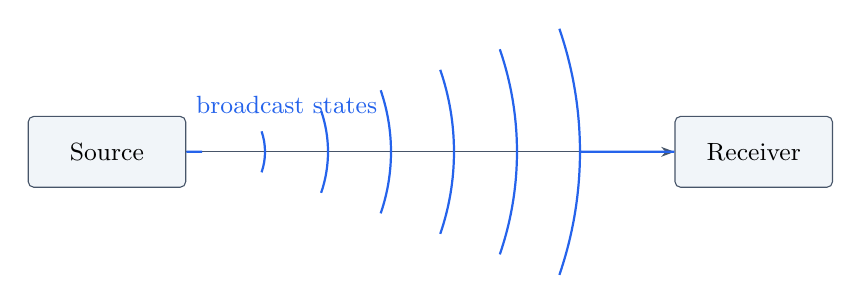
\begin{tikzpicture}[
  >=Stealth,
  stage/.style={draw=stagegray,fill=stagefill,rounded corners=2pt,
    minimum width=2cm,minimum height=9mm},
  every node/.style={font=\small}
]
  \node[stage] (source) {Source};
  \node[stage,right=6.2cm of source] (receiver) {Receiver};
  \draw[stagegray,-Stealth] (source.east) -- (receiver.west);
  \draw[signalblue,line width=.8pt,decorate,
    decoration={expanding waves,segment length=8mm,angle=19,
      pre length=2mm,post length=5mm}]
    (source.east) -- (receiver.west);
  \node[signalblue,above=6mm of source.east,anchor=west] {broadcast states};
\end{tikzpicture}
\end{document}
